\subsection{Balanceo y morfología}
La intención de esta sección es ver tanto cómo se comporta el OCR al contar con una base de datos de entrenamiento totalmente balanceada y desbalanceada como la morfología de los dígitos y qué consecuencias pueden traer. Como tal no realizaremos iteraciones sobre el alpha o el k, asumiendo valores fijos iguales a los ``mejores'' encontrados en las secciones anteriores.

En la tabla \ref{tab:totalDigitos} se puede ver la cantidad por digitos del dataset completo. Como el 5 (del que menos hay) tiene 3795 instancias, no podemos elegir más de esa cantidad. En todos los experimentos que siguen vamos a utilizar 3795 instancias, 2277 de entrenamiento y 1518 de validación.

\begin{table}[h]
\centering
\begin{tabular}{|c|c|}
\hline
0 & 4132 \\ \hline
1 & 4684 \\ \hline
2 & 4177 \\ \hline
3 & 4351 \\ \hline
4 & 4072 \\ \hline
5 & 3795 \\ \hline
6 & 4137 \\ \hline
7 & 4401 \\ \hline
8 & 4063 \\ \hline
9 & 4188 \\ \hline
\end{tabular}
\caption{Cantidad de instancias por dígito}
\label{tab:totalDigitos}
\end{table}

Primero vimos qué pasaba al tener un conjunto de entrenamiento totalmente balanceado. Como podemos ver en la fig.\ref{fig:bal_recall_prec} el sistema tiene bastante buena precisión y recall para cada una de las clases, con un accuracy de 0.925.
\begin{figure}[h]
    \centering
    \begin{subfigure}{.5\textwidth}
        \centering
        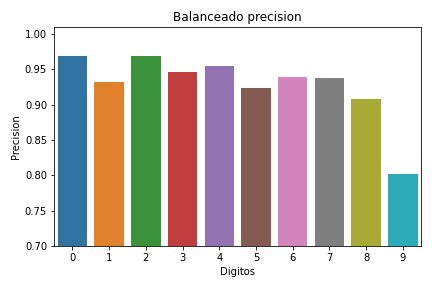
\includegraphics[width=.9\linewidth]{images/balanceo/Balanceado precision_3795.png}
    \end{subfigure}%
    \begin{subfigure}{.5\textwidth}
        \centering
        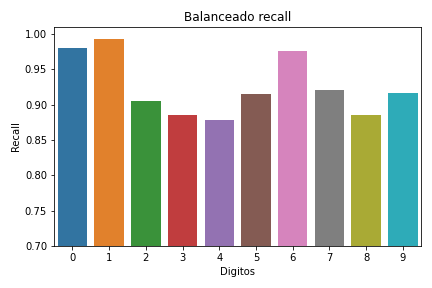
\includegraphics[width=.9\linewidth]{images/balanceo/Balanceado recall_3795.png}
    \end{subfigure}%
    \caption{Recall y precision de balanceado}
    \label{fig:bal_recall_prec}
\end{figure}

Como la precisión del 9 es la más baja intentamos mejorar esto agregando más instancias del mismo, cabe aclarar que cuando decimos agregar es en realidad un desbalance pero tenemos la misma cantidad de instancias de entrenamiento. La proporción normalizada de 9s es 0.16 y 0.093 para el resto. En la figura \ref{fig:9s_recall_prec} se ve que, contrario a lo que suponíamos, la precisión baja aún más y además empeora el recall de los 4s.
\begin{figure}[h]
    \centering
    \begin{subfigure}{.5\textwidth}
        \centering
        \includegraphics[width=.9\linewidth]{images/balanceo/Con más 9s precision_3795.png}
    \end{subfigure}%
    \begin{subfigure}{.5\textwidth}
        \centering
        \includegraphics[width=.9\linewidth]{images/balanceo/Con más 9s recall_3795.png}
    \end{subfigure}%
    \caption{Recall y precision de desbalance con más 9s}
    \label{fig:9s_recall_prec}
\end{figure}

Pero si esto es así entonces \textit{¿Qué pasa si agregamos más 4s en vez de 9s?}. Al hacer el intento, con proporción normalizada de 0.16 para los 4s y 0.093 para el resto, vimos que mejora el recall para el 4 sin bajar tanto el del 9 y obtiene mejor accuracy general, esto se puede ver en la figura \ref{fig:4s_recall_prec}.
\begin{figure}[h]
    \centering
    \begin{subfigure}{.5\textwidth}
        \centering
        \includegraphics[width=.9\linewidth]{images/balanceo/Con más 4s precision_3795.png}
    \end{subfigure}%
    \begin{subfigure}{.5\textwidth}
        \centering
        \includegraphics[width=.9\linewidth]{images/balanceo/Con más 4s recall_3795.png}
    \end{subfigure}%
    \caption{Recall y precision de desbalance con más 9s}
    \label{fig:4s_recall_prec}
\end{figure}


Esto tiene sentido, ya que el mayor error está cuando los valores son 4s pero clasifica erroneamente como 9, como se puede ver en \ref{fig:bal_conf}. Por ende al tener más instancias de 4s le estamos dando al sistema más vecinos para comparar del valor con el que más flaquea, esto aumenta el recall del 4 al dar menos falsos negativos, luego como el valor predecido era 9 la precisión de este último aumenta ya que hay menos falsos positivos.
\begin{figure}[h]
 \centering
 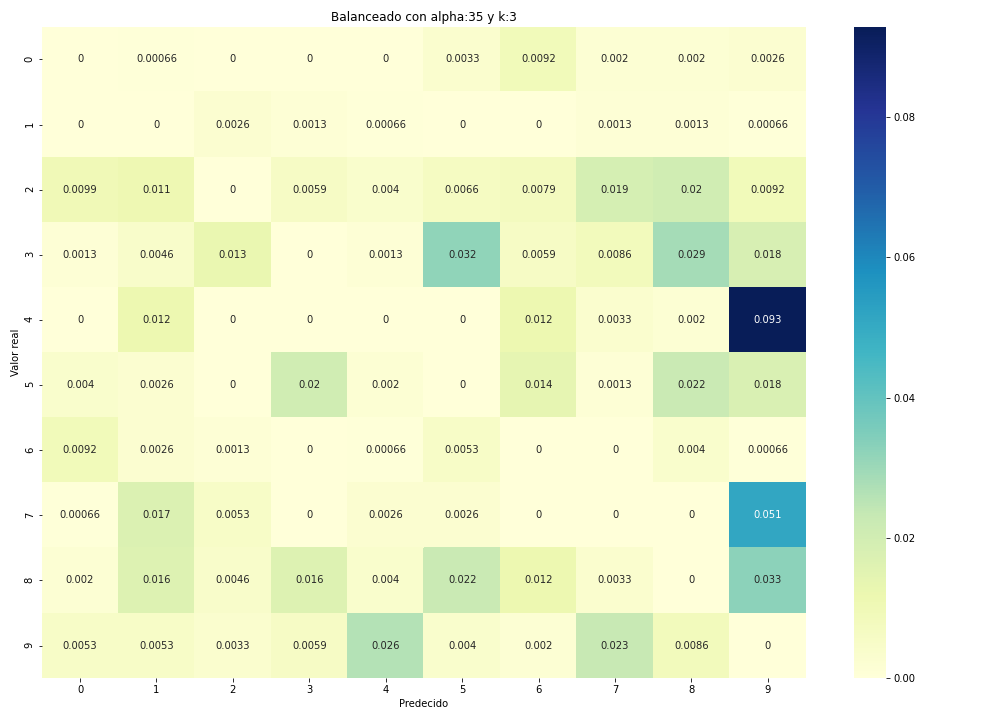
\includegraphics[width=0.8\linewidth]{images/balanceo/Balanceado con alpha:35 y k:3_3795.png}
 \caption{Matriz de confusión para dataset balanceado (diagonal anulada)}
 \label{fig:bal_conf}
\end{figure}

Creemos que los errores se deben a la morfología de estos números, ya que basta redondear un poco la línea del cuatro para que se confundan. De hecho, mirando a mano las imágenes con las cuáles comete errores podemos ver casos como [REF] y [REF] donde los 4s parecen 9.%TODO agregar imgs ejemplo

Hasta ahora sabemos que el desbalance no es inherentemente malo sino que podría beneficiarnos, entonces surge la pregunta \textit{¿Cuál es la configuración (proporciones de dígitos) que más accuracy genera?}

Para empeza desbalanceamos a mano utilizando como guía el recall de cada clase, en favor de los que menos poseen. Probamos con las proporciones: 

\begin{description}
 \item [Muchos 4s, más 3s] proporción de 0.11, 0.15 para el 3 y 4 (resp.) y 0.093 para el resto. 
 \item [Muchos 4s, más 3s, 7s y 8s] proporción de 0.15 para el 4, 0.11 para el 3,7 y 8 y 0.087 para el resto. 
\end{description}

En la figura \ref{fig:acc} se ve que con más 4s y 3s se obtiene aún más accuracy pero ya al desbalancear 7s y 8s volvemos a perder exactitud, aunque aún es mejor que el set balanceado.
\begin{figure}[h]
 \centering
 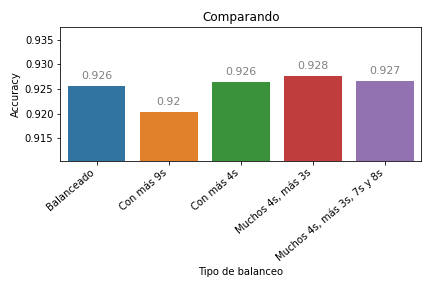
\includegraphics[width=0.65\linewidth]{images/balanceo/acc.png}
 \caption{Accuracy para cada uno de los casos.}
 \label{fig:acc}
\end{figure}



%TODO en realidad hacer el exp no?


